\documentclass[11pt]{beamer}
\usetheme{Warsaw}
\usepackage[utf8]{inputenc}
\usepackage{amsmath}
\usepackage{amsfonts}
\usepackage{amssymb}
\author{José Jácome}
\title{Introducción}
%\setbeamercovered{transparent} 
%\setbeamertemplate{navigation symbols}{} 
%\logo{} 
%\institute{} 
%\date{} 
%\subject{} 
\begin{document}

\begin{frame}
\titlepage
\end{frame}

%\begin{frame}
%\tableofcontents
%\end{frame}

\begin{frame}{Historia}

\begin{center}
\textbf{Pierre Simon Laplace}
\end{center}

\textit{Beaumont-en-Auge (Normandía) (1749) - París(1827)} fue un astrónomo, físico y matemático francés que inventó y desarrolló la transformada de Laplace y la ecuación de Laplace. Su trabajo se baso en la Mecánica Celeste (la cual le tomo cinco volumenes) también Ecuaciones Diferenciales y estudio de Probabilidades, fue estudiante de Jean d'Alembert, entre sus estudiantes destacan Siméon Denis Poisson y Joseph Fourier, fue conocido como el Newton de Francia, otro discípulo de él fue Napoleón.
\begin{center}
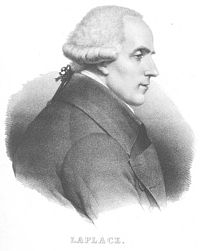
\includegraphics[scale=1.2]{Laplace.jpg}
\end{center}
\end{frame}

\begin{frame}{Introducción a la Ecuación de Laplace}
Se denomina \textit{Ecuación de Laplace} a la expresión de una ecuación en derivadas parciales de segundo orden de tipo elíptico, es usado por las necesidades de la mecánica newtoniana y tiene muchas aplicación en otras ramas d ela física teórica (astronomía, electrostática, mecánica de fluidos, mecánica cuántica)

\end{frame}

\end{document}